\documentclass[landscape,a4paper]{extarticle}
\usepackage{relsize}
\usepackage{caption}
\usepackage{multicol}
\usepackage[top=2em,bottom=2em,left=2em,right=2em]{geometry}
\usepackage[framemethod=tikz]{mdframed}
\usepackage{microtype}
\usepackage{pdfpages}
\usepackage{amsmath, amssymb, amsthm}
\usepackage{gensymb}
\usepackage{anyfontsize}
\usepackage[shortlabels]{enumitem}
\usepackage{graphicx, float}
\usepackage{ulem}
\usepackage{xcolor}
\usepackage{tgschola}

\let\bar\overline
\setlength{\columnsep}{0.7em}

% Configure image directory
\graphicspath{{../images/}}

\newenvironment{Figure}
  {\noindent\minipage{\linewidth}}
  {\endminipage\par\medskip}

% Remove caption labels
\captionsetup{labelformat=empty,labelsep=none}

% No paragraph indent
\setlength{\parindent}{0pt}

% No spaces between list items
\setlist[enumerate]{nosep, leftmargin=*}
\setlist[itemize]{nosep, leftmargin=*}

\newcommand{\sgn}{\text{sgn}}
\newcommand{\rect}[1]{\operatorname{rect}\left(#1\right)}
\newcommand{\sinc}[1]{\operatorname{sinc}\left(#1\right)}

\newcommand{\T}{\textbf{T}}

\newcommand{\lap}[1]{\mathcal{L}\left\{#1\right\}}
\newcommand{\invlap}[1]{\mathcal{L}^{-1}\left\{#1\right\}}

\newcommand{\fourier}[1]{\Im\left\{#1\right\}}
\newcommand{\invfourier}[1]{\Im^{-1}\left\{#1\right\}}

% No spaces before and after math mode
\expandafter\def\expandafter\normalsize\expandafter{%
    \normalsize%
    \setlength\abovedisplayskip{0pt}%
    \setlength\belowdisplayskip{0pt}%
    \setlength\abovedisplayshortskip{-8pt}%
    \setlength\belowdisplayshortskip{2pt}%
}

\begin{document}
\fontsize{6}{8}\selectfont
\fontfamily{qcs}\selectfont
\begin{multicols*}{5}
    % \textbf{Euler's formula}
    % \begin{align*}
    %     e^{j\theta}=\cos(\theta) + j\sin(\theta)\\
    %     e^{-j\theta}=\cos(\theta)-j\sin(\theta)
    % \end{align*}

    \textbf{\uline{Chapter 1}}

    \textbf{1.2.2 Bounded signals}

    $x(t)$ is bounded if 

    $\exists M\ [(0 < M < \infty) \wedge (\forall t\ |x(t)| \leq M)]$

    (got upper n lower range limit)

    \textbf{1.2.3 Absolutely integrable signals}

    $x(t)$ is absolutely integrable if 
    \[
        \int_{-\infty}^{\infty}|x(t)| dt < \infty
    \]

    % \textbf{1.2.4 Periodc and aperiodic signals}

    % Periodic: there is a non-zero positive value, $T$, satisfying 
    % \[
    %     x(t)=x(t+T) \ \forall t \tag{1.1}
    % \]

    % Aperiodic: not periodic

    \textbf{1.2.6 Energy and Power Signals}

    \textbf{Energy signals}
    \[
        E = \int_{-\infty}^{\infty}|x(t)|^2 dt \tag{1.3a}
    \]
    
    \[
        x(t) \text{ is an energy signal} \iff 0 < E < \infty \tag{1.3b}
    \]
    \textbf{Power signals}
    \[
        P = \lim_{\tau \to \infty}\frac{1}{2\tau}\int_{-\tau}^{\tau}|x(t)|^2dt \tag{1.4a}
    \]

    \[
        x(t) \text{ is a power signal} \iff 0 < P < \infty \tag{1.4b}
    \]
    If $x(t)$ is a periodic signal, average power may be computed by
    \[
        \frac{1}{T}\int_0^T|x(t)|^2 dt
    \]
    \begin{itemize}
        \item Energy signals have 0 average power, bc E = finite implies P = 0
        \item Power signals have infinite total energy, bc P = finite implies $E = \infty$
        \item All bounded periodic signals are power signals
    \end{itemize}
    \textbf{u(t):}

    \begin{Figure}
        \centering
        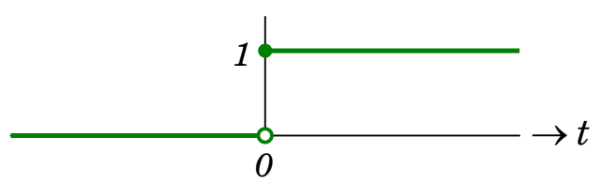
\includegraphics[width=0.8\linewidth]{unitStep.png}
    \end{Figure}

    \textbf{sgn(t):}

    \begin{Figure}
        \centering
        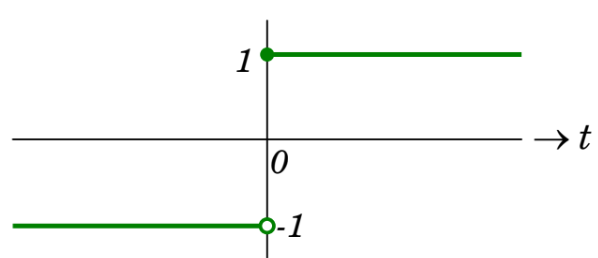
\includegraphics[width=0.8\linewidth]{signum.png}
    \end{Figure}

    \textbf{rect$\left( \frac{t}{T}\right)$:}

    \begin{Figure}
        \centering
        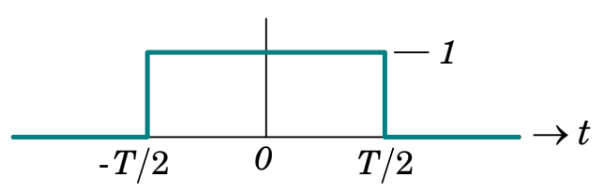
\includegraphics[width=0.8\linewidth]{rect.png}
    \end{Figure}

    \textbf{tri$\left( \frac{t}{T}\right)$:}

    \begin{Figure}
        \centering
        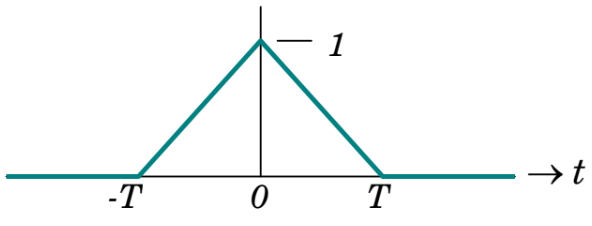
\includegraphics[width=0.8\linewidth]{tri.png}
    \end{Figure}

    \textbf{sinc$\left(\frac{t}{T}\right)$:}

    \begin{Figure}
        \centering
        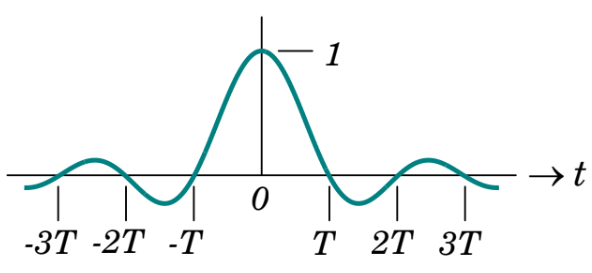
\includegraphics[width=0.8\linewidth]{sinc.png}
    \end{Figure}

    \textbf{$e^{-\alpha t}u(t)$: }

    \begin{Figure}
        \centering
        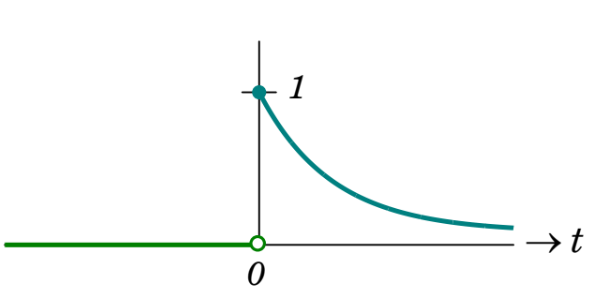
\includegraphics[width=0.8\linewidth]{rightSidedDecayingExp.png}
    \end{Figure}

    \textbf{$e^{-\alpha |t|}$: }

    \begin{Figure}
        \centering
        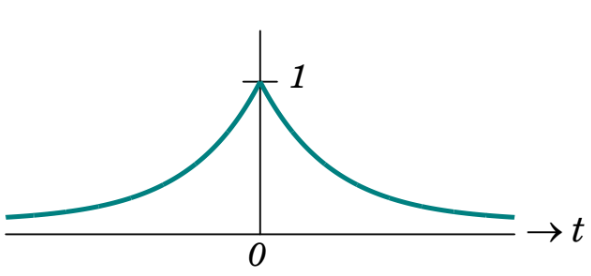
\includegraphics[width=0.8\linewidth]{twoSidedDecayingExp.png}
    \end{Figure}
    % \textbf{Sinusoidal signals}
    % \begin{align*}
    %     x(t)&=\mu \cos(\omega_0t+\phi)\\
    %     &= \mu\cos(2\pi f_0t + \phi)\\
    %     &= \mu\cos(\frac{2\pi t}{T} + \phi)
    % \end{align*} \newline
    % \[
    %     T_0=\frac{2\pi}{\omega_0}=\frac{1}{f_0}
    % \]

    \textbf{\uline{Chapter 2}}

    \textbf{2.1 Time-domain Operations}

    % \textbf{2.1.1 Time-Scaling}

    % $x(\alpha t)$: Scale x-axis by a factor of $\frac{1}{\alpha}$

    % $x(-t)$: Reflect about x-axis

    % \textbf{2.1.2 Time-Shifting}

    % $x(t-\beta)$:

    % $\beta > 0$: Delaying $x(t)$ by $\beta$ units of time (translate right along x-axis)

    % $\beta > 0$: Advancing $x(t)$ by $\beta$ units of time (translate left along x-axis)

    \textbf{2.1.5 Convolution of 2 Signals}

    $x(t)*y(t)=\int_{-\infty}^{\infty}x(\alpha)y(t-\alpha)\ d\alpha$

    % \textbf{Properties of convolutions}
    % \begin{enumerate}
    %     \item Commutative: $f * g = g * f$
    %     \item Associative: $f * (g * h) = (f * g) * h$
    %     \item Distributive: $f * (g + h) = (f * g) + (f * h)$
    % \end{enumerate}

    \textbf{Properties of Dirac-$\delta$: }
    \begin{enumerate}
        \item Symmetry:
        \[
            \delta(t)=\delta(-t) \tag{2.3}
        \]
        \item Sampling: 
        \[
            x(t)\delta(t-\lambda)=x(\lambda)\delta(t-\lambda) \tag{2.4}
        \]
        \item Sifting
        \begin{align*}
            \int_{-\infty}^{\infty} x(t)\delta(t-\lambda)dt=x(\lambda) \tag{2.5}
        \end{align*}
        \item Replication
        \begin{align*}
            x(t)*\delta(t-\lambda)=x(t-\lambda) \tag{2.6}
        \end{align*}
    \end{enumerate}
    % \textbf{2.2.1 Dirac-$\delta$ Comb function}
    % \begin{align*}
    %     &\sum_{n=-\infty}^{\infty}\delta(t-nT)\\
    %     &= \ldots+\delta(t+T)+\delta(t)+\delta(t-T) + \ldots
    % \end{align*}

    \textbf{Convolution with Dirac-$\delta$ Comb function}
    \begin{align*}
        x_p(t)&=x(t)*\sum_n\delta(t-nT)\\
        &=\sum_n x(t-nT)
    \end{align*}

    \textbf{Multiplication with the Dirac-$\delta$ Comb function}

    Used for sampling
    \begin{align*}
        x_s(t)&=x(t)\times\sum_n\delta(t-nT)\\
        &=\sum_nx(t)\times\delta(t-nT)\\
        &=\sum_nx(nT)\delta(t-nT)
    \end{align*}
    
    \textbf{\uline{Chapter 3}}

    \textbf{3.2 Spectrum of a Sinusoid}

    \textbf{Spectrum of a Complex Exponential Signal}
    \[
        \tilde{x}(t)=\mu e^{j(2\pi f_0t+\phi)} = \mu e^{j\phi} \times e^{j2\pi f_0t},
    \]
    % where $\mu$: magnitude spectrum, $\phi$: phase spectrum, $f_0$: frequency

    \textbf{Spectrum of a Cosine Signal}
    \begin{align*}
        &\mu \cos(2\pi f_0t + \phi)\\
        % = \ &\frac{\mu}{2}e^{j\phi}e^{j2\pi f_0t} + \frac{\mu}{2} \mu e^{-j\phi}e^{-j2\pi f_0t}\\
        = \ &\frac{\mu}{2}e^{j\phi}e^{j2\pi f_0t} + \frac{\mu}{2}  e^{j(-\phi)}e^{j2\pi (-f_0)t}
    \end{align*}\\
    \textbf{Spectrum of a Sine Signal}
    \begin{align*}
        \mu\sin(2\pi f_0 t + \phi)
        % =\ &\frac{\mu}{2}e^{j(\phi - 0.5\pi)}e^{j2\pi f_0t} + \frac{\mu}{2}e^{-j(\phi-0.5\pi)}e^{j2\pi (-f_0)t}\\
        =\ &\frac{\mu}{2}e^{j(\phi - 0.5\pi)}e^{j2\pi f_0t} \\
        + \ &\frac{\mu}{2}e^{j(-\phi+0.5\pi)}e^{j2\pi (-f_0)t}
    \end{align*}
    \textbf{Complex exponential Fourier Series}
    \begin{align*}
        x_p(t)&=\sum_{k=-\infty}^{\infty}c_ke^{j2\pi kt/T_p}\\
        &=\sum_{k=-\infty}^{\infty}c_ke^{j2\pi kf_pt} \tag{3.1a}
    \end{align*}
    \begin{align*}
        c_k=\frac{1}{T_p}\int_{t_0}^{t_0+T_p}x_p(t)e^{-j2\pi kt/T_p}dt, k \in \mathbb{Z} \tag{3.1b}
    \end{align*}

    \textbf{Trigonometric Fourier Series}
    \begin{align*}
        x_p(t) = \ a_0 + 2\sum_{k=1}^{\infty} [ &a_k \cos(2\pi kt/T_p) \\
        &+ b_k \sin(2\pi kt/T_p)]
    \end{align*}
    \begin{align*}
        a_k&=\frac{1}{T_p}\int_{t_0}^{t_0+T_p}x_p(t)\cos(2\pi kt/T_p)dt; k \geq 0\\
        b_k&=\frac{1}{T_p}\int_{t_0}^{t_0+T_p}x_p(t)\sin(2\pi kt/T_p)dt; k > 0
        \tag{3.2}
    \end{align*}

    \textbf{\uline{Chapter 4}}\\
    % \textbf{Dirichlet Conditions}\\
    % Conditions for existence of Fourier Transform:
    % \begin{enumerate}
    %     \item $x(t)$ has only a finite number of maxima and minima in any finite time interval
    %     \item $x(t)$ has only a finite number of discontinuities in any finite time interval
    %     \item $x(t)$ is absolutely integrable
    % \end{enumerate}
    % 3 is weak Dirichlet condition: satisfied by most energy signals, violated by all power signals.\\
    \textbf{4.1 Fourier Transform}\\
    \textbf{Forward Fourier Transform}
    \[
        X(f)=\int_{-\infty}^{\infty}x(t)e^{-j2\pi ft}dt \tag{4.1a}
    \]
    \textbf{Inverse Fourier Transform}
    \[
       x(t)=\int_{-\infty}^{\infty}X(f)e^{j2\pi ft}df \tag{4.1b} 
    \]

    \textbf{Spectrum of exponentially decaying pulse}
    \begin{align*}
        x(t) &= Ae^{-\alpha t} u(t)\\
        % & = \begin{cases}
        %     Ae^{-\alpha t}; &t > 0\\
        %     0; &t < 0
        % \end{cases}\\
        &\text{Assume } \alpha > 0
    \end{align*}

    \[
        X(f) = \frac{A}{\alpha + j 2\pi f}
    \]

    % \textbf{4.2 Properties of Fourier Transform}
    % \begin{itemize}
    %     \item $X(f)=\Im\{x(t)\}$ denotes the Fourier transform of $x(t)$
    %     \item $x(t)={\Im}^{-1}\{X(f)\}$ denotes the inverse Fourier transform of $X(f)$
    %     \item $x(t) \rightleftarrows X(f)$ denotes a Fourier transform pair with the time-domain on the LHS and frequency-domain on the RHS.
    % \end{itemize}
    % \textbf{Linearity}

    % If $x_1(t) \rightleftarrows X_1(f)$ and $x_2(t) \rightleftarrows X_2(f)$, then \[
    %     \alpha x_1(t) + \beta x_2(t)\rightleftarrows \alpha X_1(f) + \beta X_2 (f) \tag{4.2}
    % \]

    % \textbf{Time Scaling}

    % \[
    %     x(\beta t) \rightleftarrows \frac{1}{|\beta|} X\left( \frac{f}{\beta}\right) \tag{4.3}
    % \]

    % \textbf{Duality}

    % \[
    %     X(t) \rightleftarrows x(-f) \tag{4.4}
    % \]

    % \centerline{or}

    % \[
    %     X(-t) \rightleftarrows x(f)
    % \]

    % \textbf{Time Shifting}

    % \[
    %     x(t-t_0) \rightleftarrows X(f)e^{-j2\pi ft_0} \tag{4.5}
    % \]

    % \[
    %     x(t+t_0) \rightleftarrows X(f)e^{j 2 \pi f t_0}
    % \]

    % \textbf{Frequency Shifting (Modulation)}

    % \[
    %     x(t)e^{j2\pi f_0t} \rightleftarrows X(f-f_0) \tag{4.6}
    % \]

    % \[
    %     x(t)e^{-j2\pi f_0t} \rightleftarrows X(f+f_0)
    % \]

    % \textbf{Differentiation in the Time Domain}

    % \[
    %     \frac{d}{dt}x(t) \rightleftarrows j2\pi f \cdot X(f) \tag{4.7}
    % \]

    % \textbf{Integration in the Time Domain}

    % \[
    %     \int_{-\infty}^{t}x(\tau)\ d\tau \rightleftarrows \frac{1}{j2\pi f}X(f) + \frac{1}{2}X(0)\delta(f) \tag{4.8}
    % \]

    % \textbf{Convolution in the Time Domain / Multiplication in the Frequency Domain}
    % \begin{align*}
    %     &x_1(t) * x_2(t) \\
    %     = &\int_{-\infty}^{\infty}x_1(\alpha)x_2(t-\alpha)\ d\alpha \rightleftarrows X_1(f)X_2(f) \tag{4.9a}
    % \end{align*}

    % \textbf{Multiplication in the Time Domain / Convolution in the Frequency Domain} 
    % \begin{align*}
    %     x_1(t)x_2(t) \rightleftarrows &\int_{-\infty}^{\infty} X_1(\alpha)X_2(f-\alpha)\ d\alpha \\=&X_1(f)*X_2(f) \tag{4.9b}
    % \end{align*}

    \textbf{4.3 Spectral properties of a REAL signal}
    \begin{itemize}
        \item If $x(t)$ is \textbf{REAL} ($x^*(t)=x(t)$), then
        \begin{itemize}
            \item $X(f)$ is conjugate symmetric \textcolor{black!70}{($X^*(f)=X(f)$)}
            \item $|X(f)|$ is even \textcolor{black!70}{($|X(f)|=|X(-f)|$)}
            \item $\angle X(f)$ is odd \textcolor{black!70}{($\angle X(f)=-\angle X(-f)$)}
        \end{itemize}
        \item If $x(t)$ is \textbf{REAL} and \textbf{EVEN} ($x^*(t)=x(t) \wedge x(-t)=x(t)$), then
        \begin{itemize}
            \item $X(f)$ is real \textcolor{black!70}{($X^*f=X(f)$)}
            \item $X(f)$ is even \textcolor{black!70}{($X(-f)=X(f)$)}
        \end{itemize}
        \item If $x(t)$ is \textbf{REAL} and \textbf{ODD} ($x^*(t)=x(t) \wedge x(-t)=-x(t)$), then
        \begin{itemize}
            \item $X(f)$ is imaginary \textcolor{black!70}{($X^*(f) = -X(f)$)}
            \item $X(f)$ is odd \textcolor{black!70}{($X(-f)=-X(f)$)}
        \end{itemize}
    \end{itemize}

    The above can apply to Fourier series coefficients of periodic signals too:
    \begin{itemize}
        \item $x_p(t)$ is \textbf{REAL}
        \begin{itemize}
            \item $c_k$ is conjugate symmetric \textcolor{black!70}{($c_k^* = c_{-k}$)}
            \item $|c_k|$ has even symmetry \textcolor{black!70}{($|c_k|=|c_{-k}|$)}
            \item $\angle c_k$ has odd symmetry \textcolor{black!70}{($\angle c_k = -\angle c_{-k}$)}
        \end{itemize}
        \item $x_p(t)$ is \textbf{REAL} and \textbf{EVEN}
        \begin{itemize}
            \item $c_k$ is real \textcolor{black!70}{($c_k^*=c_k$)}
            \item $c_k$ is even \textcolor{black!70}{($c_k=c_{-k}$)}
        \end{itemize}
        \item $x_p(t)$ is \textbf{REAL} and \textbf{ODD}
        \begin{itemize}
            \item $c_k$ is imaginary \textcolor{black!70}{($c_k^*=-c_k$)}
            \item $c_k$ is odd \textcolor{black!70}{($c_k=-c_{-k}$)}
        \end{itemize}
    \end{itemize}
    \textbf{4.4 Spectrum of Signals that are not Absolutely Integrable}

    \[
        \Im\{K\delta (t)\} = \int_{-\infty}^{\infty}K \delta(t)e^{-j2\pi  ft}dt=K \tag{4.13}
    \]

    By duality, $\Im\{K\}=K\delta(f)$
    % \begin{Figure}
    %     \centering
    %     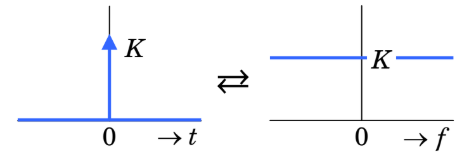
\includegraphics[width=0.8\linewidth]{fourierOfImpulse.png}
    % \end{Figure}
    % \begin{Figure}
    %     \centering
    %     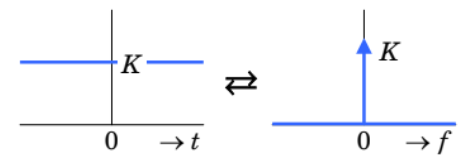
\includegraphics[width=0.8\linewidth]{fourierOfConstant.png}
    % \end{Figure}

    \textbf{4.4.1 Spectrm of Unit Step and Signum function}

    \[
        \Im\{u(t)\}=\frac{1}{j2\pi f} + \frac{1}{2}\delta(f)
    \]

    \[
        \Im\{\text{Sgn}(t)\} = \frac{1}{j\pi f}
    \]

    \textbf{4.4.2 Continuous-Frequency Spectrum of Periodic Signals}

    The following make use of the fact that
    \[
        \Im\{k\}=K\delta(f) \tag{4.14}
    \]
    \textbf{DC}
    \begin{align*}
        &x_{dc}(t)=K \\
        &X_{dc}(f)=\Im\{k\}=K\Im\{1\}=K\delta(f)
    \end{align*}
    % \begin{Figure}
    %     \centering
    %     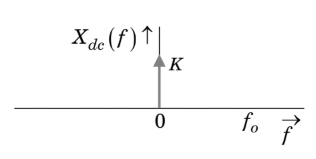
\includegraphics[width=0.8\linewidth]{continuousSpectrum_DC.png}
    % \end{Figure}    
    \textbf{Complex Exponential}
    \begin{align*}
        &\tilde{x}(t) = Ke^{j2\pi f_0t} \\
        &\tilde{X}(f)=\Im\{Ke^{j2\pi f_0t}\} = K\delta(f-f_0)
    \end{align*}
    % \begin{Figure}
    %     \centering
    %     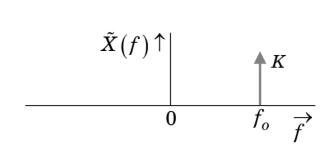
\includegraphics[width=0.8\linewidth]{continuousSpectrum_complexExponential.png}
    % \end{Figure}
    \textbf{Cosine}
    \begin{align*}
        &\Im\{K\cos{(2\pi f_0t)}\}\\
        =&\frac{K}{2}\delta(f-f_0)+\frac{K}{2}\delta(f+f_0)
    \end{align*}
    % \begin{Figure}
    %     \centering
    %     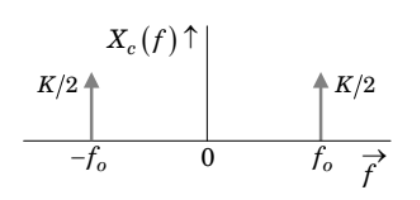
\includegraphics[width=0.8\linewidth]{continuousFreqSpectrum_Cos.png}
    % \end{Figure}
    \textbf{Sine}
    \begin{align*}
        &\Im\{K\sin(2\pi f_0 t)\}\\
        = &\frac{K}{j2}\delta(f-f_0) - \frac{K}{j2}\delta(f+f_0)
    \end{align*}

    \[
    \text{where } \begin{cases}
            |X_s(f)|&=\frac{K}{2}\delta(f-f_0)\\
            &\quad+ \ \frac{K}{2}\delta(f+f_0)\\\\
            \angle X_s(f)&= \begin{cases}
                -\pi/2, &\quad f=f_0\\
                \pi/2, &\quad f=-f_0
            \end{cases}
        \end{cases}
    \]

    % \begin{Figure}
    %     \centering
    %     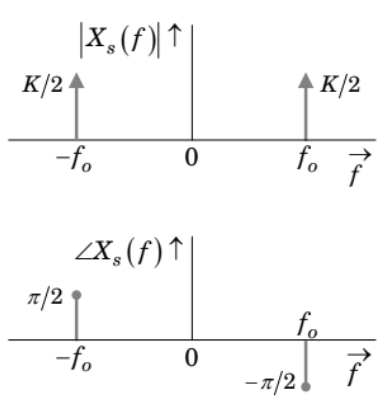
\includegraphics[width=0.8\linewidth]{continuousFreqSpectrum_Sine.png}
    % \end{Figure}

    \textbf{Arbitrary periodic signals}

    Let $x_p(t)$ be a periodic signal with period $T_p$ and fundamental frequency $f_p$
    \[
        X_p(f)=\sum_{k=-\infty}^{\infty}c_k\delta (f-kf_p) \tag{4.16} 
    \]
    % \begin{Figure}
    %     \centering
    %     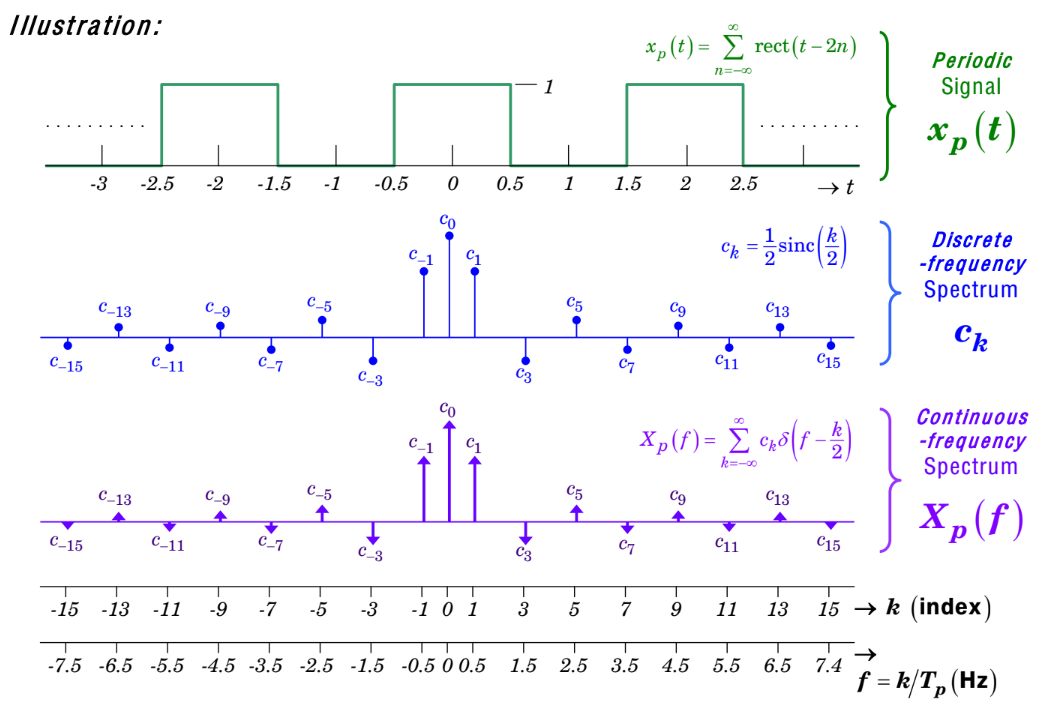
\includegraphics[width=\linewidth]{continuousFreqSpectrum_periodic.png}
    % \end{Figure}

    \textbf{4.4.2.1 Spectrum of Dirac-$\delta$ Comb function}

    \[
        \text{comb}_\lambda(t) \triangleq \sum_n\delta(t-n\lambda)
    \]

    % \begin{Figure}
    %     \centering
    %     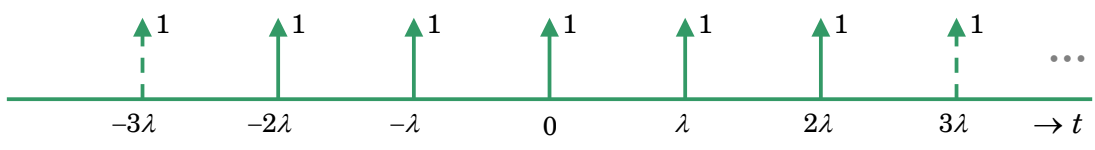
\includegraphics[width=\linewidth]{comb.png}
    % \end{Figure}

    \[
        c_k=\frac{1}{\lambda}
    \]
    % \begin{Figure}
    %     \centering
    %     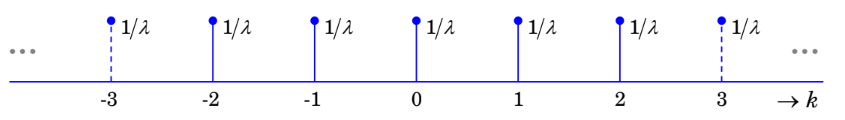
\includegraphics[width=\linewidth]{discreteFreqSpec_comb.png}
    % \end{Figure}
    \begin{align*}
        \Im\{\text{comb}_\lambda(t)\} &= \text{COMB}_\lambda(f)\\
        &=\frac{1}{\lambda}\sum_k\delta(f-k/\lambda)
    \end{align*}
    % \begin{Figure}
    %     \centering
    %     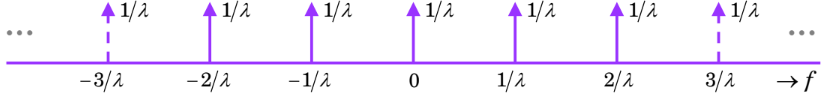
\includegraphics[width=\linewidth]{continuousFreqSpectrum_comb.png}
    % \end{Figure}
    
    \textbf{\uline{Chapter 5}}

    \textbf{5.1 Energy Spectral Density (ESD)}

    Total energy of a signal $x(t)$ is defined as 
    \[
        E=\int_{-\infty}^{\infty}|x(t)|^2 dt \text{ (Joules)} \tag{5.1}
    \]
    \textbf{Rayleigh Energy Theorem}
    \[
        E=\int_{-\infty}^{\infty}|x(t)|^2dt=\int_{-\infty}^{\infty}|X(f)|^2df \tag{5.2},
    \]

    \textbf{Energy Spectral Density}
    \[
        E_x(f)=|X(f)|^2 \text{ Joules Hz}^{-1}\tag{5.3}
    \]
    \textbf{Properties of $E_x(f)$}
    \begin{enumerate}
        \item $E_x(f)$ is a real function of $f$
        \item $E_x(f) \geq 0 \quad\forall f$
        \item $E_x(f)$ is an even function of $f$ if $x(t)$ is real.
    \end{enumerate}

    \textbf{5.2 Power Spectral Density (PSD)}

    In the time-domain, the average power of a signal $x(t)$ is defined as 
    \[
        P=\lim_{\tau \to \infty} \frac{1}{2\tau}\int_{-\tau}^{\tau}|x(t)|^2 dt \tag{5.4}
    \]
    Windowed version of $x(t)$:
    \[
        x_W(t)=x(t)\text{rect}\left(\frac{t}{2W}\right) \tag{5.5}
    \]
    \textbf{Parseval Power Theorem}
    \begin{align*}
        P&=\lim_{W \to \infty}\frac{1}{2W}\int_{-W}^{W}|x(t)|^2dt\\
        &=\int_{-\infty}^{\infty}\lim_{W \to \infty}\frac{1}{2W}|X_W(f)|^2df \tag{5.9}
    \end{align*}
    \textbf{Power Spectral Density}
    \[
        {P_x(f)=\lim_{W \to \infty}\frac{1}{2W}|X_W(f)|^2} \text{ Watts Hz}^{-1} \tag{5.10}
    \]
    \textbf{Properties of $P_x(f)$}
    \begin{enumerate}
        \item $P_x(f)$ is a real function of $f$
        \item $P_x(f) \geq 0 \quad \forall f$
        \item $P_x(f)$ is an even function of $f$ if $x(t)$ is real.
    \end{enumerate}

    \textbf{5.2.1 PSD of Periodic Signals}

    From chapter 4 equation 4.16:
    \[
        X_p(f)=\sum_{k=-\infty}^{\infty}c_k \delta (f-kf_p)
    \]
    \textbf{PSD of $x_p(t)$}
    \[
        P_x(f)=\sum_{k=-\infty}^{\infty}|c_k|^2\delta (f-kf_p) \tag{5.12}
    \]
    \textbf{Average power of $x_p(t)$}
    \[
        P=\int_{-\infty}^{\infty}P_x(f)df=\sum_{k=-\infty}^{\infty}|c_k|^2 \tag{5.13}
    \]
    \textbf{5.3 Bandwidth}

    \textbf{5.3.1 Bandlimited Signals}

    \textbf{Lowpass signal}

    % A signal $x(t)$ is said to be a bandlimited lowpass signal if its magnitude spectrum is concentrated around 0 Hz, and at the same time satisfies
    % \[
    %     |X(f)|=0; \quad |f| > B \tag{5.14}
    % \]
    % where B is defined as the bandwidth of the signal. 
    \begin{Figure}
        \centering
        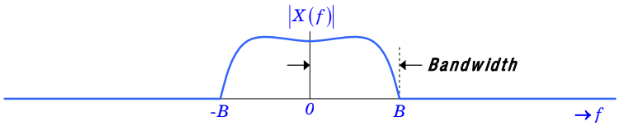
\includegraphics[width=\linewidth]{bandlimitedLowpassSignal.png}
    \end{Figure}
    \textbf{Bandpass signal}

    % A signal $x(t)$ is said to be a bandlimited bandpass signal if its magnitude spectrum is concentrated around a non-zero center frequency $f_c$, and at the same time satisfies \[
    %     |X(f)|=0; \quad ||f|-f_c|>B/2 \tag{5.15}
    % \]
    % where B is defined as the bandwidth of the signal
    \begin{Figure}
        \centering
        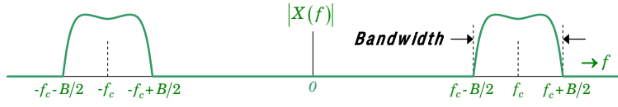
\includegraphics[width=\linewidth]{bandlimitedBandpassSignal.png}
    \end{Figure}
    \textbf{5.3.2 Signals with Unrestricted Band}

    \textbf{5.3.2.1 3dB Bandwidth}

    \textbf{Lowpass signal:}
    % The frequency where $|X(f)|=|X(0)|/\sqrt{2}$ first occurs (or where $|X(f)|^2=|X(0)|^2/2$ first occurs) when $f$ is increased from 0 Hz.
    \begin{Figure}
        \centering
        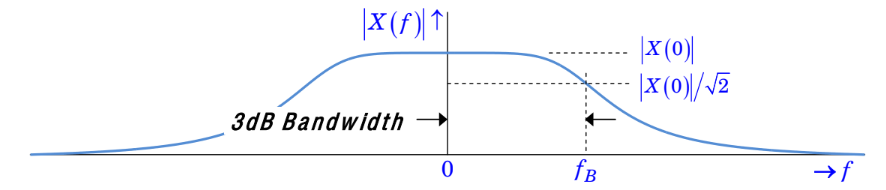
\includegraphics[width=\linewidth]{3dB_lowpass.png}
    \end{Figure}

    \textbf{Bandpass signal:}
    \begin{Figure}
        \centering
        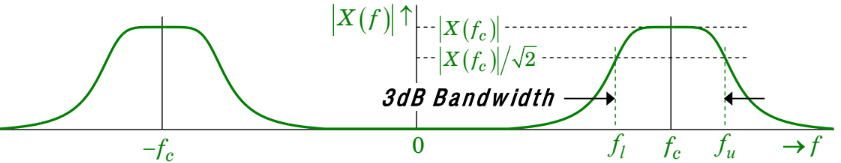
\includegraphics[width=\linewidth]{3dB_bandpass.png}
    \end{Figure}
    
    \textbf{5.3.2.2 1st-null Bandwidth}

    \textbf{Lowpass signal: } 
    % The frequency at which $|X(f)|=0$ first occurs when $f$ is increased from 0 Hz:
    \begin{Figure}
        \centering
        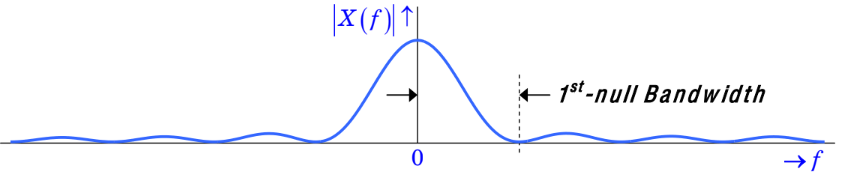
\includegraphics[width=\linewidth]{1stNull_lowpass.png}
    \end{Figure}
    \textbf{Bandpass signal: }
    \begin{Figure}
        \centering
        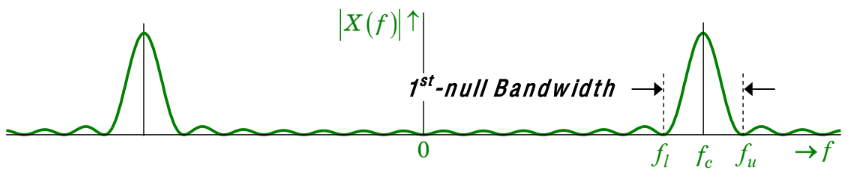
\includegraphics[width=\linewidth]{1stNull_bandpass.png}
    \end{Figure}

    \textbf{5.3.2.3 M\% Energy Containment Bandwidth}

    Smallest bandwidth that contains at least M\% of the total signal energy $E = \int_{-\infty}^{\infty}E_x(f)\ df$

    \textbf{Lowpass:}
    \begin{Figure}
        \centering
        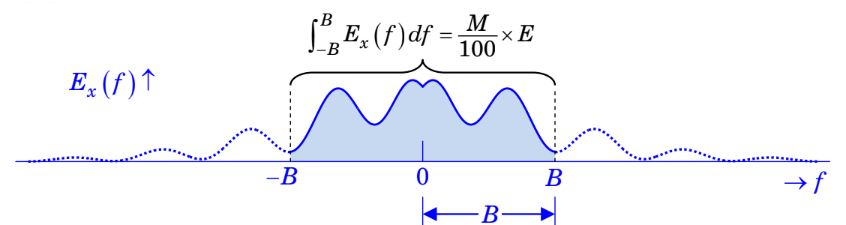
\includegraphics[width=\linewidth]{MPercentEnergy_lowpass.png}
    \end{Figure}
    \textbf{Bandpass:}
    \begin{Figure}
        \centering
        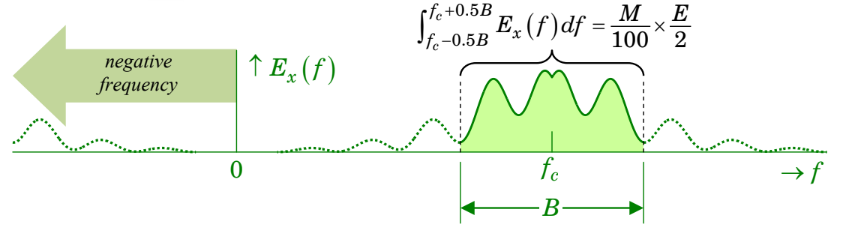
\includegraphics[width=\linewidth]{MPercentEnergy_bandpass.png}
    \end{Figure}

    \textbf{5.3.2.4 M\% Power Containment Bandwidth}

    The smallest bandwidth that contains at least M\% of the average signal power. For a periodic signal, the aerage power is given by
    \[
        P = \int_{-\infty}^{\infty}P_x(f)df=\sum_{k=-\infty}^{\infty}|c_k|^2
    \]
    where $f_p$(Hz) is the fundamental frequency and $c_k$'s are the Fourier series coefficients.
    \begin{Figure}
        \centering
        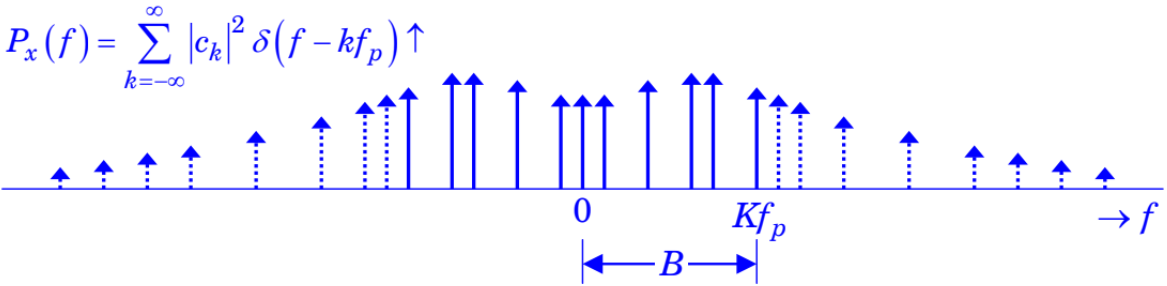
\includegraphics[width=\linewidth]{MPercentPower.png}
    \end{Figure}
    \[
        B = Kf_p
    \]
    where $K$ is the smallest positive integer that satisfies 
    \[
        \sum_{k=-k}^{K}|c_k|^2 \geq \frac{M}{100} \times P
    \]

    \textbf{\uline{Chapter 6}}

    \textbf{6.1 Systems}

    % \begin{itemize}
    %     \item A system is a mathematical model of a physical process that relates the input (or excitation) signal to the output (or response) signal.
    %     \item With an input $x(t)$ and an output $y(t)$, the system may be viewed as a transformation (or mapping) of $x(t)$ into $y(t)$, mathematically expressed as 
    %     \[
    %         y(t) = \textbf{T}\left[x(t)\right] \tag{6.1}
    %     \]
    % \end{itemize}

    \textbf{6.2 Classification of Systems}

    \textbf{6.2.1 Systems with Memory and Without Memory}

    Memoryless: output at a given time is dependent on only the input at that time.

    Otherwise, the system has memory / is dynamic.

    \textbf{6.2.2 Causal and Noncausal Systems}

    Causal (or non-anticipative): Its output, $y(t)$, at the present time depends on only the present and/or past values of its input, $x(t)$.

    $\therefore$ not possible for a causal system to produce an output before an input is applied. $\therefore \forall t < 0\ y(t)=0$.

    \textbf{6.2.3 Stable and Unstable Systems}

    BIBO stable (bounded-input/bounded-output): For every bounded input $x(t)$ where

    \[
        \forall t\ |x(t)| \leq k \tag{6.2}
    \]

    the system produces a bounded output $y(t)$ where 

    \[
        \forall t\ |y(t)| \leq L \tag{6.3}
    \]
    in which $K$ and $L$ are positive constants.

    \textbf{6.2.4 Linear and Nonlinear Systems}

    Linear system satisfies the following:
    \begin{align}
        \begin{split}
            &\T[\alpha_1x_1(t) + \alpha_2x_2(t)]\\
            =&\ \alpha_1\T[x_1(t)] + \alpha_2\T[x_2(t)]\\
            =&\ \alpha_1y_1(t) + \alpha_2y_2(t)
        \end{split} \tag{6.6}
    \end{align}

    (6.6) is known as the superposition property.

    Important property of linear systems: 
    
    $x(t) = 0 \implies y(t) = 0$

    \textbf{6.2.5 Time-Invariant and Time-Varying Systems}

    Time-invariant: a time shift (delay or advance) in the input signal, $x(t)$, causes the same time shift in the output signal, $y(t)$.

    \[
        \T[x(t-\tau)] = y(t-\tau) \tag{6.7}
    \]

    A time-varying system is one which does not satisfy (6.7).

    \textbf{Laplace Transform}

    \[
        \tilde{F}(s) = \lap{f(t)} = \int_{0}^{\infty}f(t)e^{-st} dt \tag{6.8}
    \]
    where $s$ is a complex variable.

    \textbf{Inverse Laplace Transform}
    \[
        f(t) = \invlap{\tilde{F}(s)} = \frac{1}{2\pi j} \int_{\gamma - j \infty}^{\gamma + j \infty}\tilde{F}(s)ds \tag{6.9}
    \]
    
    % TODO: solving linear differential equation

    \textbf{\uline{Chapter 7}}

    \textbf{7.1 Impulse Response}

    Impulse response, $h(t)$: The response/output when the input is a unit impulse, $\delta(t)$.
    \[
        \delta(t) \rightarrow \text{LTI system} \rightarrow h(t)
    \]
    where 

    \[
        h(t) = \T[\delta(t)] \tag{7.1}
    \]

    % From replication property, 

    % \begin{align*}
    %     x(t) = x(t) * \delta (t) = \int_{-\infty}^{\infty}x(\tau)\delta(t-\tau) d\tau \tag{7.2}
    % \end{align*}

    % Substituting (7.2) into (6.1), 
    % \begin{align*}
    %     \begin{split}
    %         y(t) &= \T[x(t)]\\
    %         &= \T\left[\int_{-\infty}^{\infty}x(\tau)\delta(t-\tau) d\tau\right]\\
    %         &= \int_{-\infty}^{\infty}x(\tau)\T[\delta(t-\tau)]d\tau
    %     \end{split} \tag{7.3}
    % \end{align*}

    % As the system is time-invariant, by applying (6.7) to (7.1),

    % \[
    %     h(t-\tau) = \T\left[\delta(t-\tau)\right] \tag{7.4}
    % \]

    % Sub (7.4) into (4.3):
    % \begin{align*}
    %     \begin{split}
    %         y(t) &= \int_{-\infty}^{\infty}x(\tau)h(t-\tau) d\tau\\
    %         &= x(t) * h(t)
    %     \end{split} 
    %     \tag{7.5}
    % \end{align*}

    % Therefore
    \[
        \T[x(t)] = y(t) = x(t) * h(t) \tag{7.5}
    \]

    \textbf{7.1.1 Step Response}

    Step response: the output of the system when input is unit step function
    \begin{align*}
        u(t) \rightarrow h(t) \rightarrow o(t) &= \int_{-\infty}^{\infty}h(\tau) u(t-\tau) d \tau\\
        &= \int_{-\infty}^{t}h(\tau) d \tau
    \end{align*}

    Step response equals integration of impulse response:
    \[
        o(t) = \int_{-\infty}^{t}h(\tau) d\tau
    \]

    Impulse response equals differentiation of step response:
    \[
        h(t) = \frac{d}{dt} o(t)
    \]

    \textbf{7.2 Frequency Response}

    Frequency response ($H(f)$): The Fourier transform of the system impulse response $h(t)$
    \[
        H(f) = \fourier{h(t)} = \int_{-\infty}^{\infty} h(t) e^{-j2\pi ft} dt \tag{7.6}
    \]
    \begin{align*}
        Y(f) &= X(f) \cdot H(f) \tag{7.7}
    \end{align*}

    % \begin{Figure}
    %     \centering
    %     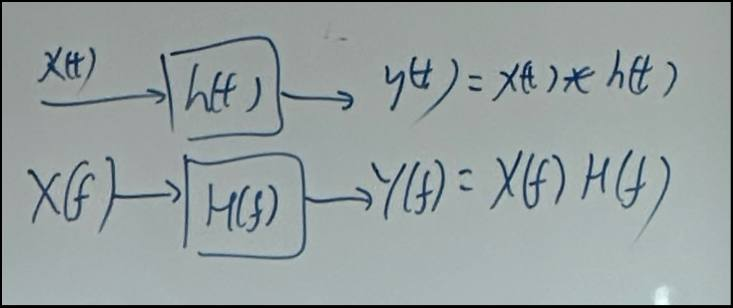
\includegraphics[width=0.6\linewidth]{LTI_hf_ht.jpg}
    % \end{Figure}

    \[
        H(f) = |H(f)| e^{j \angle H(f)} \tag{7.8}
    \]

    where $|H(f)|$ is called the magnitude response and $\angle H(f)$ is called the phase response of the system.

    \textbf{7.3 Transfer Function}

    Transfer function $\tilde{H}(s)$: Laplace transform of $h(t)$
    \[
        \tilde{H}(s) = \lap{h(t)} = \int_{0}^{\infty}h(t) e^{-st} dt \tag{7.9}
    \]

    where $s = \sigma + j \omega$ is a complex variable.
    \begin{align*}
        y(t) &= x(t) * h(t)\\
        \tilde{Y}(s) &= \tilde{X}(s) \cdot \tilde{H}(s) \tag{7.10}
    \end{align*}
    \begin{Figure}
        \centering
        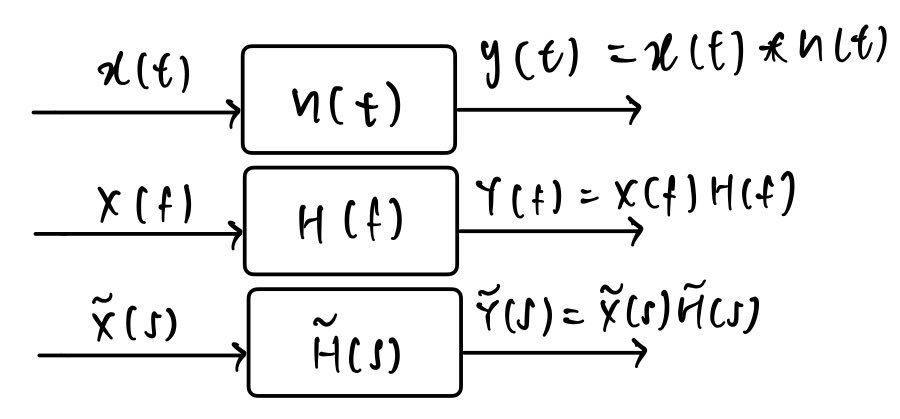
\includegraphics[width=0.7\linewidth]{LTI_ht_hf_hs.jpg}        
    \end{Figure}

    \textbf{7.4 Relationship between Transfer Function and Frequency Response}

    Substituting $s = j \omega$ into (7.9), we get 
    \[
        \left.\tilde{H}(s)\right|_{s=j\omega} = \tilde{H}(j \omega) = \int_{0}^{\infty}h(t)e^{-j \omega t} dt \tag{7.11}
    \]

    Sub $\omega = 2 \pi f$ into (7.11):
    \[
        \left.\tilde{H}(j\omega)\right|_{\omega = 2\pi f} = \int_{0}^{\infty} h(t) e^{-j2\pi f t}dt \tag{7.12}
    \]

    For causal LTI systems, $\forall t < 0\ h(t) = 0$. Hence (7.6) and (7.12) are equivalent.
    \[
        H(f) = \left.\tilde{H}(j \omega)\right|_{\omega=2\pi f} \tag{7.13}
    \]

    \begin{Figure}
        \centering
        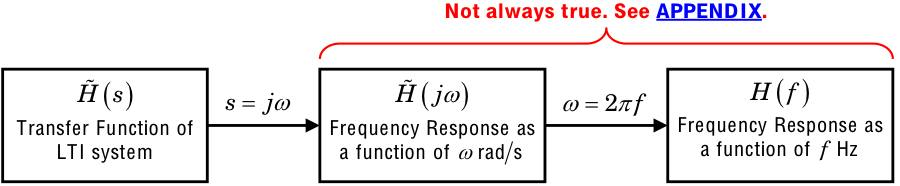
\includegraphics[width=\linewidth]{transferFunc_freqResponse.jpg}        
    \end{Figure}

    \[
        \tilde{H}(j\omega) = |\tilde{H}(j\omega)|e^{j\angle \tilde{H}(j \omega)} \tag{7.14}
    \]

    where $|\tilde{H}(j \omega)|$ is called the magnitude response
    and $\angle \tilde{H}(j \omega)$ is called the phase response of the system.

    \textbf{7.4 Sinusoidal Response at Steady-State}

    Let system input at steady-state be 
    
    \[
        x(t) = Ae^{j (2\pi f_0t + \psi)} \tag{7.15}
    \]

    Then

    \[
        X(f) = Ae^{j\psi}\delta (f-f_0) \tag{7.16}
    \]

    \[
        Y(f) = A \left|H(f_0)\right|e^{j(\psi + \angle H(f_0))}\delta(f-f_0) \tag{7.17}
    \]

    \begin{align*}
        \begin{split}
            y(t) &= \invfourier{Y(f)}\\
            &= A \left|H(f_0)\right|e^{j(2\pi f_0 t + \psi + \angle H(f_0))} 
        \end{split} \tag{7.18}
    \end{align*}

    \begin{Figure}
        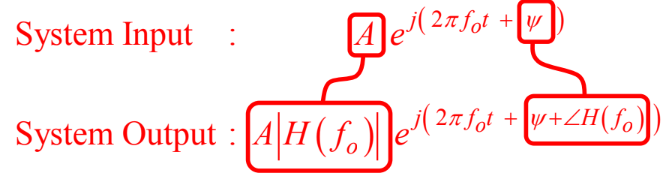
\includegraphics[width=0.8\linewidth]{sinusoidalResponseComparison.png}        
    \end{Figure}

    \begin{Figure}
        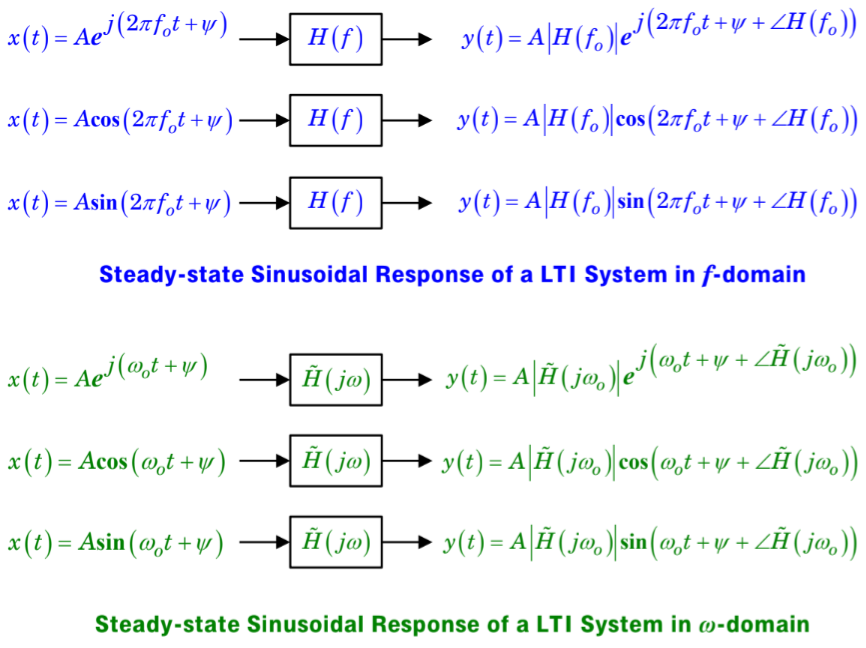
\includegraphics[width=\linewidth]{sinusoidalResponse.png}        
    \end{Figure}

    \textbf{7.6 LTI Systems Described by Differential Equations}

    LTI systems represented by linear constant-coefficient differential equations have the general form
    \[
        \sum_{n=0}^{N}a_n \frac{d^ny(t)}{dt^n} = \sum_{m=0}^{M} b_m \frac{d^mx(t)}{dt^m} \tag{7.21}
    \]

    where $x(t)$ is input, $y(t)$ is output, and $a_n, b_m$ are real constants.

    \textbf{7.6.1 Transfer Function}

    Applying Laplace to both sides of (7.21) with initial conditions set to 0,
    \[
        \sum_{n=0}^{N}a_n \tilde{Y}(s)s^n = \sum_{m=0}^{M} b_m \tilde{X}(s)s^m \tag{7.22}
    \]

    \begin{align*}
        \begin{split}
            \tilde{H}(s) &= \frac{\tilde{Y}(s)}{\tilde{X}(s)}\\
            % &= \left( \left. \sum_{m=0}^{M}b_ms^m \right/ \sum_{n=0}^{N}a_ns^n \right) \\
            &= \frac{b_Ms^M + b_{M-1}s^{M-1} + \ldots + b_0}{a_Ns^N + a_{N-1}s^{N-1} + \ldots + a_0}
        \end{split} \tag{7.23a}
    \end{align*}

    \begin{align*}
        \begin{split}
            \tilde{H}(s) &= K\frac{\left(\frac{s}{z_1} + 1\right)\left(\frac{s}{z_2} + 1\right) \ldots \left(\frac{s}{z_M} + 1\right)}{\left(\frac{s}{p_1} + 1\right)\left(\frac{s}{p_2} + 1\right) \ldots \left(\frac{s}{p_N} + 1\right)}\\
            K &= \frac{a_0}{b_0}
        \end{split} \tag{7.23b}
    \end{align*}

    \begin{align*}
        \begin{split}
            \tilde{H}(s) &= K'\frac{(s+z_1)(s+z_2)\ldots (s+z_M)}{(s+p_1)(s+p_2)\ldots (s+p_N)} \\
            K &=  \frac{b_M}{a_N}
        \end{split} \tag{7.23c}
    \end{align*}

    $\forall n \in \{1,2, \ldots , N\}$ 
    \begin{itemize}
        % \item $-p_n$ are roots of the denominator polynomial of $\tilde{H}(s)$
        \item $\tilde{H}(-p_n) = \infty$
        \item $-p_n$ are called \textbf{poles} of $\tilde{H}(s)$
    \end{itemize}
    $\forall m \in \{1,2, \ldots , M\}$ 
    \begin{itemize}
        % \item $-z_m$ are roots of the numerator polynomial of $\tilde{H}(s)$
        \item $\tilde{H}(-z_m) = 0$
        \item $-z_m$ are called \textbf{zeros} of $\tilde{H}(s)$
    \end{itemize}

    The system is said to have $N$ poles and $M$ zeros, and the difference $N-M$ is called pole-zero excess.

    \textbf{7.6.2 System Stability}

    \textbf{BIBO Stable}
    \begin{itemize}
        \item All system poles lying on the left-half s-plane
        \item $h(t)$ will converge to 0 as $t$ tends to infinity\\
        $\lim_{t \to \infty} h(t) = 0$
    \end{itemize}

    % E.g.

    % $\tilde{H}(s) = \frac{1}{s + \alpha}$

    % Pole: $s = - \alpha$

    % $h(t) = e^{-\alpha t} u(t)$
    % \begin{Figure}
    %     \centering
    %     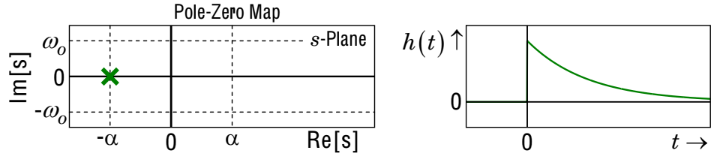
\includegraphics[width=\linewidth]{biboStable1.png}        
    % \end{Figure}

    % $\tilde{H}(s) = \frac{\omega_0}{(s + \alpha)^2 + \omega_0^2}$

    % Poles: $s_{1,2} = -\alpha \pm j\omega_0$

    % $h(t) = e^{-\alpha t} \sin (\omega_0 t) u (t)$

    % \begin{Figure}
    %     \centering
    %     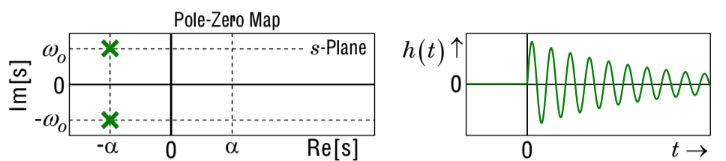
\includegraphics[width=\linewidth]{biboStable2.png}        
    % \end{Figure}

    \textbf{Marginally Stable}
    \begin{itemize}
        \item One or more \textbf{non-repeated} system poles lying on the imaginary axis of the s-plane and no system pole lying on the right half s-plane.
        \item $h(t)$ will not ``blow up'' and become unbounded, but neither will it converge to zero as $t$ tends to infinity.\\
        $\lim_{t \to \infty} |h(t)| \neq \infty$ and $\lim_{t \to \infty} h(t) \neq 0$
    \end{itemize}

    % E.g.

    % $\tilde{H}(s) = \frac{1}{s}$

    % Pole: $s = 0$

    % $h(t) = u(t)$
    % \begin{Figure}
    %     \centering
    %     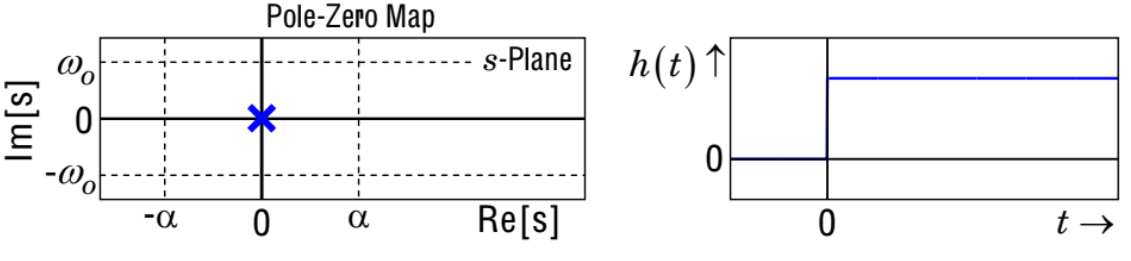
\includegraphics[width=\linewidth]{marginallyStable1.png}        
    % \end{Figure}

    % $\tilde{H}(s) = \frac{\omega_0}{s^2 + \omega_0^2}$

    % Poles: $s_{1,2} = \pm j\omega_0$

    % $h(t) = \sin (\omega_0 t) u (t)$

    % \begin{Figure}
    %     \centering
    %     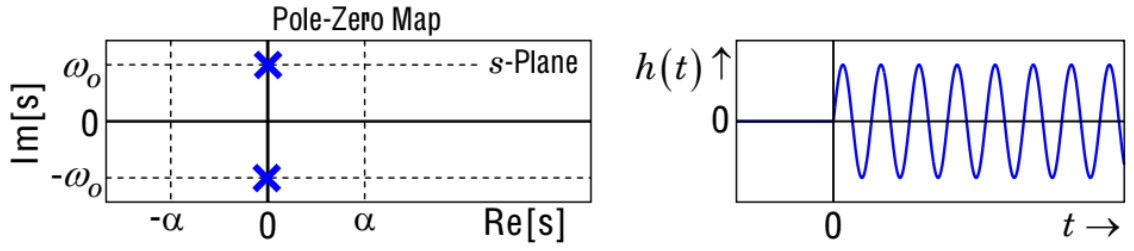
\includegraphics[width=\linewidth]{marginallyStable2.png}        
    % \end{Figure}

    \textbf{Unstable (Case 1)}
    \begin{itemize}
        \item One or more system poles lying on the right-half s-plane
        \item $h(t)$ will ``blow up'' and become unbounded as $t$ tends to infinity\\
        $\lim_{t \to \infty}|h(t)| = \infty$
    \end{itemize}

    % E.g.

    % $\tilde{H}(s) = \frac{1}{s - \alpha}$

    % Pole: $s = \alpha$

    % $h(t) = e^{\alpha t}u(t)$

    % \begin{Figure}
    %     \centering
    %     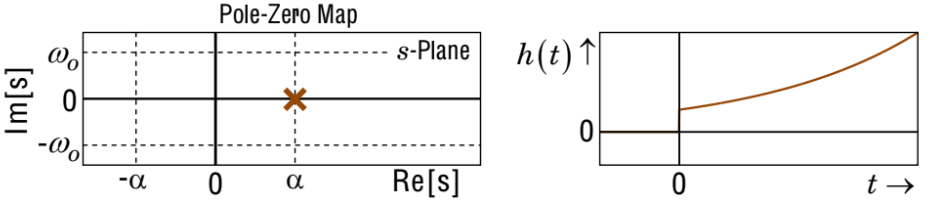
\includegraphics[width=\linewidth]{unstableCase1_1.png}        
    % \end{Figure}

    % $\tilde{H}(s) = \frac{\omega_0}{(s - \alpha)^2 + \omega_0^2}$

    % Poles: $s_{1,2} = \alpha \pm j\omega_0$

    % $h(t) = e^{\alpha t}\sin (\omega_0 t) u (t)$

    % \begin{Figure}
    %     \centering
    %     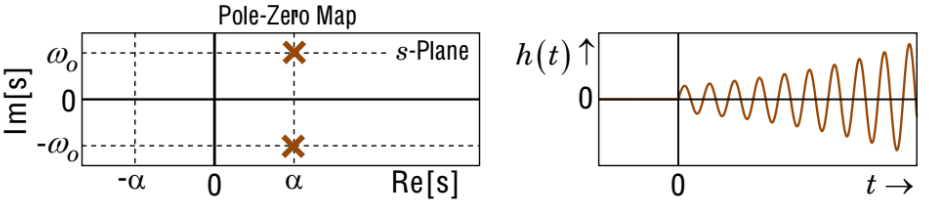
\includegraphics[width=\linewidth]{unstableCase1_2.png}        
    % \end{Figure}

    \textbf{Unstable (Case 2)}
    \begin{itemize}
        \item One or more repeated system poles lying on the imaginary axis
        \item $h(t)$ will ``blow up'' and become unbounded as $t$ tends to infinity\\
        $\lim_{t \to \infty}|h(t)| = \infty$
    \end{itemize}

    % E.g.

    % $\tilde{H}(s) = \frac{1}{s^2}$

    % Pole: $s_{1,2} = 0$

    % $h(t) = tu(t)$

    % \begin{Figure}
    %     \centering
    %     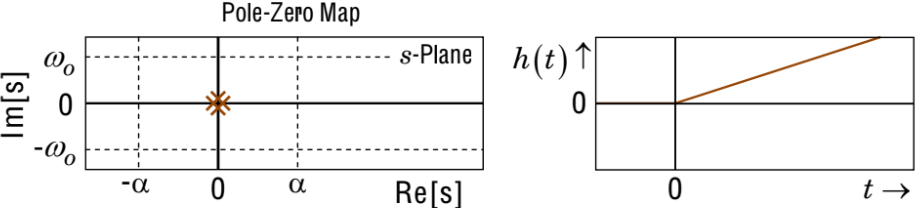
\includegraphics[width=\linewidth]{unstableCase2_1.png}        
    % \end{Figure}

    % $\tilde{H}(s) = \frac{\omega_0}{(s^2 + \omega_0^2)^2}$

    % Poles: $s_{1,2,3,4} = \pm j\omega_0, \pm j \omega_0$

    % $h(t) = \frac{1}{2} \left[\omega_0^{-1}\sin(\omega_0 t) - t \cos(\omega_0 t)\right] u(t)$

    % \begin{Figure}
    %     \centering
    %     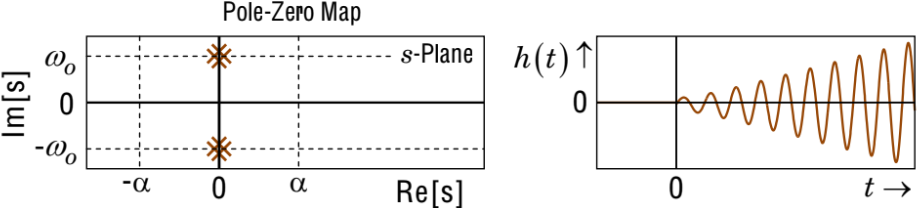
\includegraphics[width=\linewidth]{unstableCase2_2.png}        
    % \end{Figure}

    \textbf{7.7 First Order System (Standard Form)}

    \textbf{7.7.1 Differential Eqn, Transfer Func, Impulse Response and Step Response}
    \begin{itemize}
        \item Differential equation:
        \[
            T\frac{dy(t)}{dt}+y(t)=Kx(t) \tag{7.26}
        \]
        where 
        \begin{itemize}
            \item $x(t)$: system input
            \item $y(t)$: system output
            \item $K$: DC gain
            \item $T$: time-constant
        \end{itemize}
        \item Transfer Function $\tilde{H}(s)$:
        \begin{align*}
            &Ts\tilde{Y}(s) + \tilde{Y}(s) = K \tilde{X}(s)\\
            &\rightarrow \tilde{H}(s) = \frac{\tilde{Y}(s)}{\tilde{X}(s)} = \frac{K}{Ts + 1} \tag{7.27}
        \end{align*}
        Pole: $s_1$ = $-\frac{1}{T}$
        \item Impulse Response $h(t)$\\
        $h(t) = \invlap{\tilde{H}(s)} = \frac{K}{T}e^{-t/T}u(t)$
        \item Step Response $o(t)$
        \begin{align*}
            o(t) &= \int_{-\infty}^{t} h(\tau) d \tau = \invlap{\frac{1}{s}\tilde{H}(s)}\\
            &= K\left[1-e^{-t/T}\right]u(t)
        \end{align*}
    \end{itemize}

    \textbf{7.8 Second Order System (Standard Form)}
    \textbf{7.8.1 Differential Eqn and Transfer Func}
    \begin{itemize}
        \item Differential equation:
        \[
            \frac{d^2y(t)}{dt^2} + 2 \zeta \omega_n \frac{dy(t)}{dt} + \omega_n^2 y(t) = K \omega_n^2 x(t) \tag{7.28}
        \]
        where
        \begin{itemize}
            \item $x(t)$: system input
            \item $y(t)$: system output
            \item $\zeta$: damping ratio
            \item $\omega_n$: undamped natural frequency (when $\zeta < 1$)
            \item $K$: DC gain
        \end{itemize}
        \item Transfer function $\tilde{H}(s)$
        \begin{align*}
            &s^2 \tilde{Y}(s) + 2 \zeta \omega_ns\tilde{Y}(s) + \omega_n^2\tilde{Y}(s) = K \omega_n^2\tilde{X}(s)\\
            &\implies \tilde{H}(s) = \frac{\tilde{Y}(s)}{\tilde{X}(s)} = \frac{K \omega_n^2}{s^2 + 2 \zeta \omega_n s + \omega_n^2} \tag{7.29}
        \end{align*}
        Poles: $s_{1,2} = -\omega_n \zeta \pm \omega_n\left(\zeta^2 - 1\right)^{1/2}$
        % \item Damping
        % \begin{Figure}
        %     \centering
        %     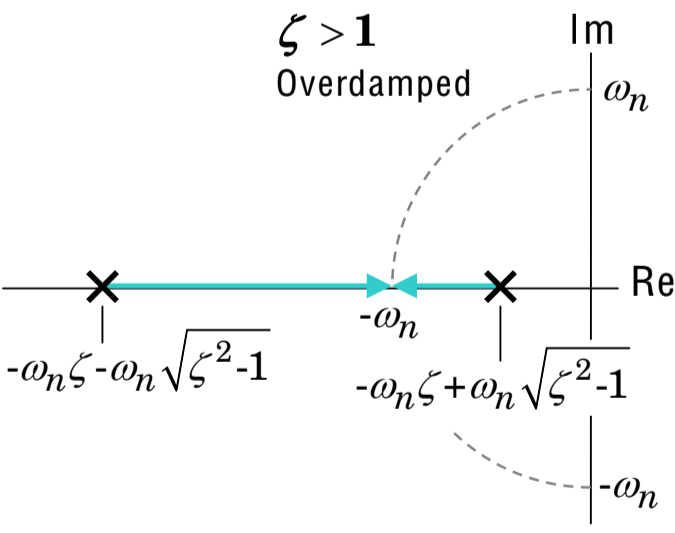
\includegraphics[width=\linewidth]{overdamped.png}                
        % \end{Figure}
        % \begin{Figure}
        %     \centering
        %     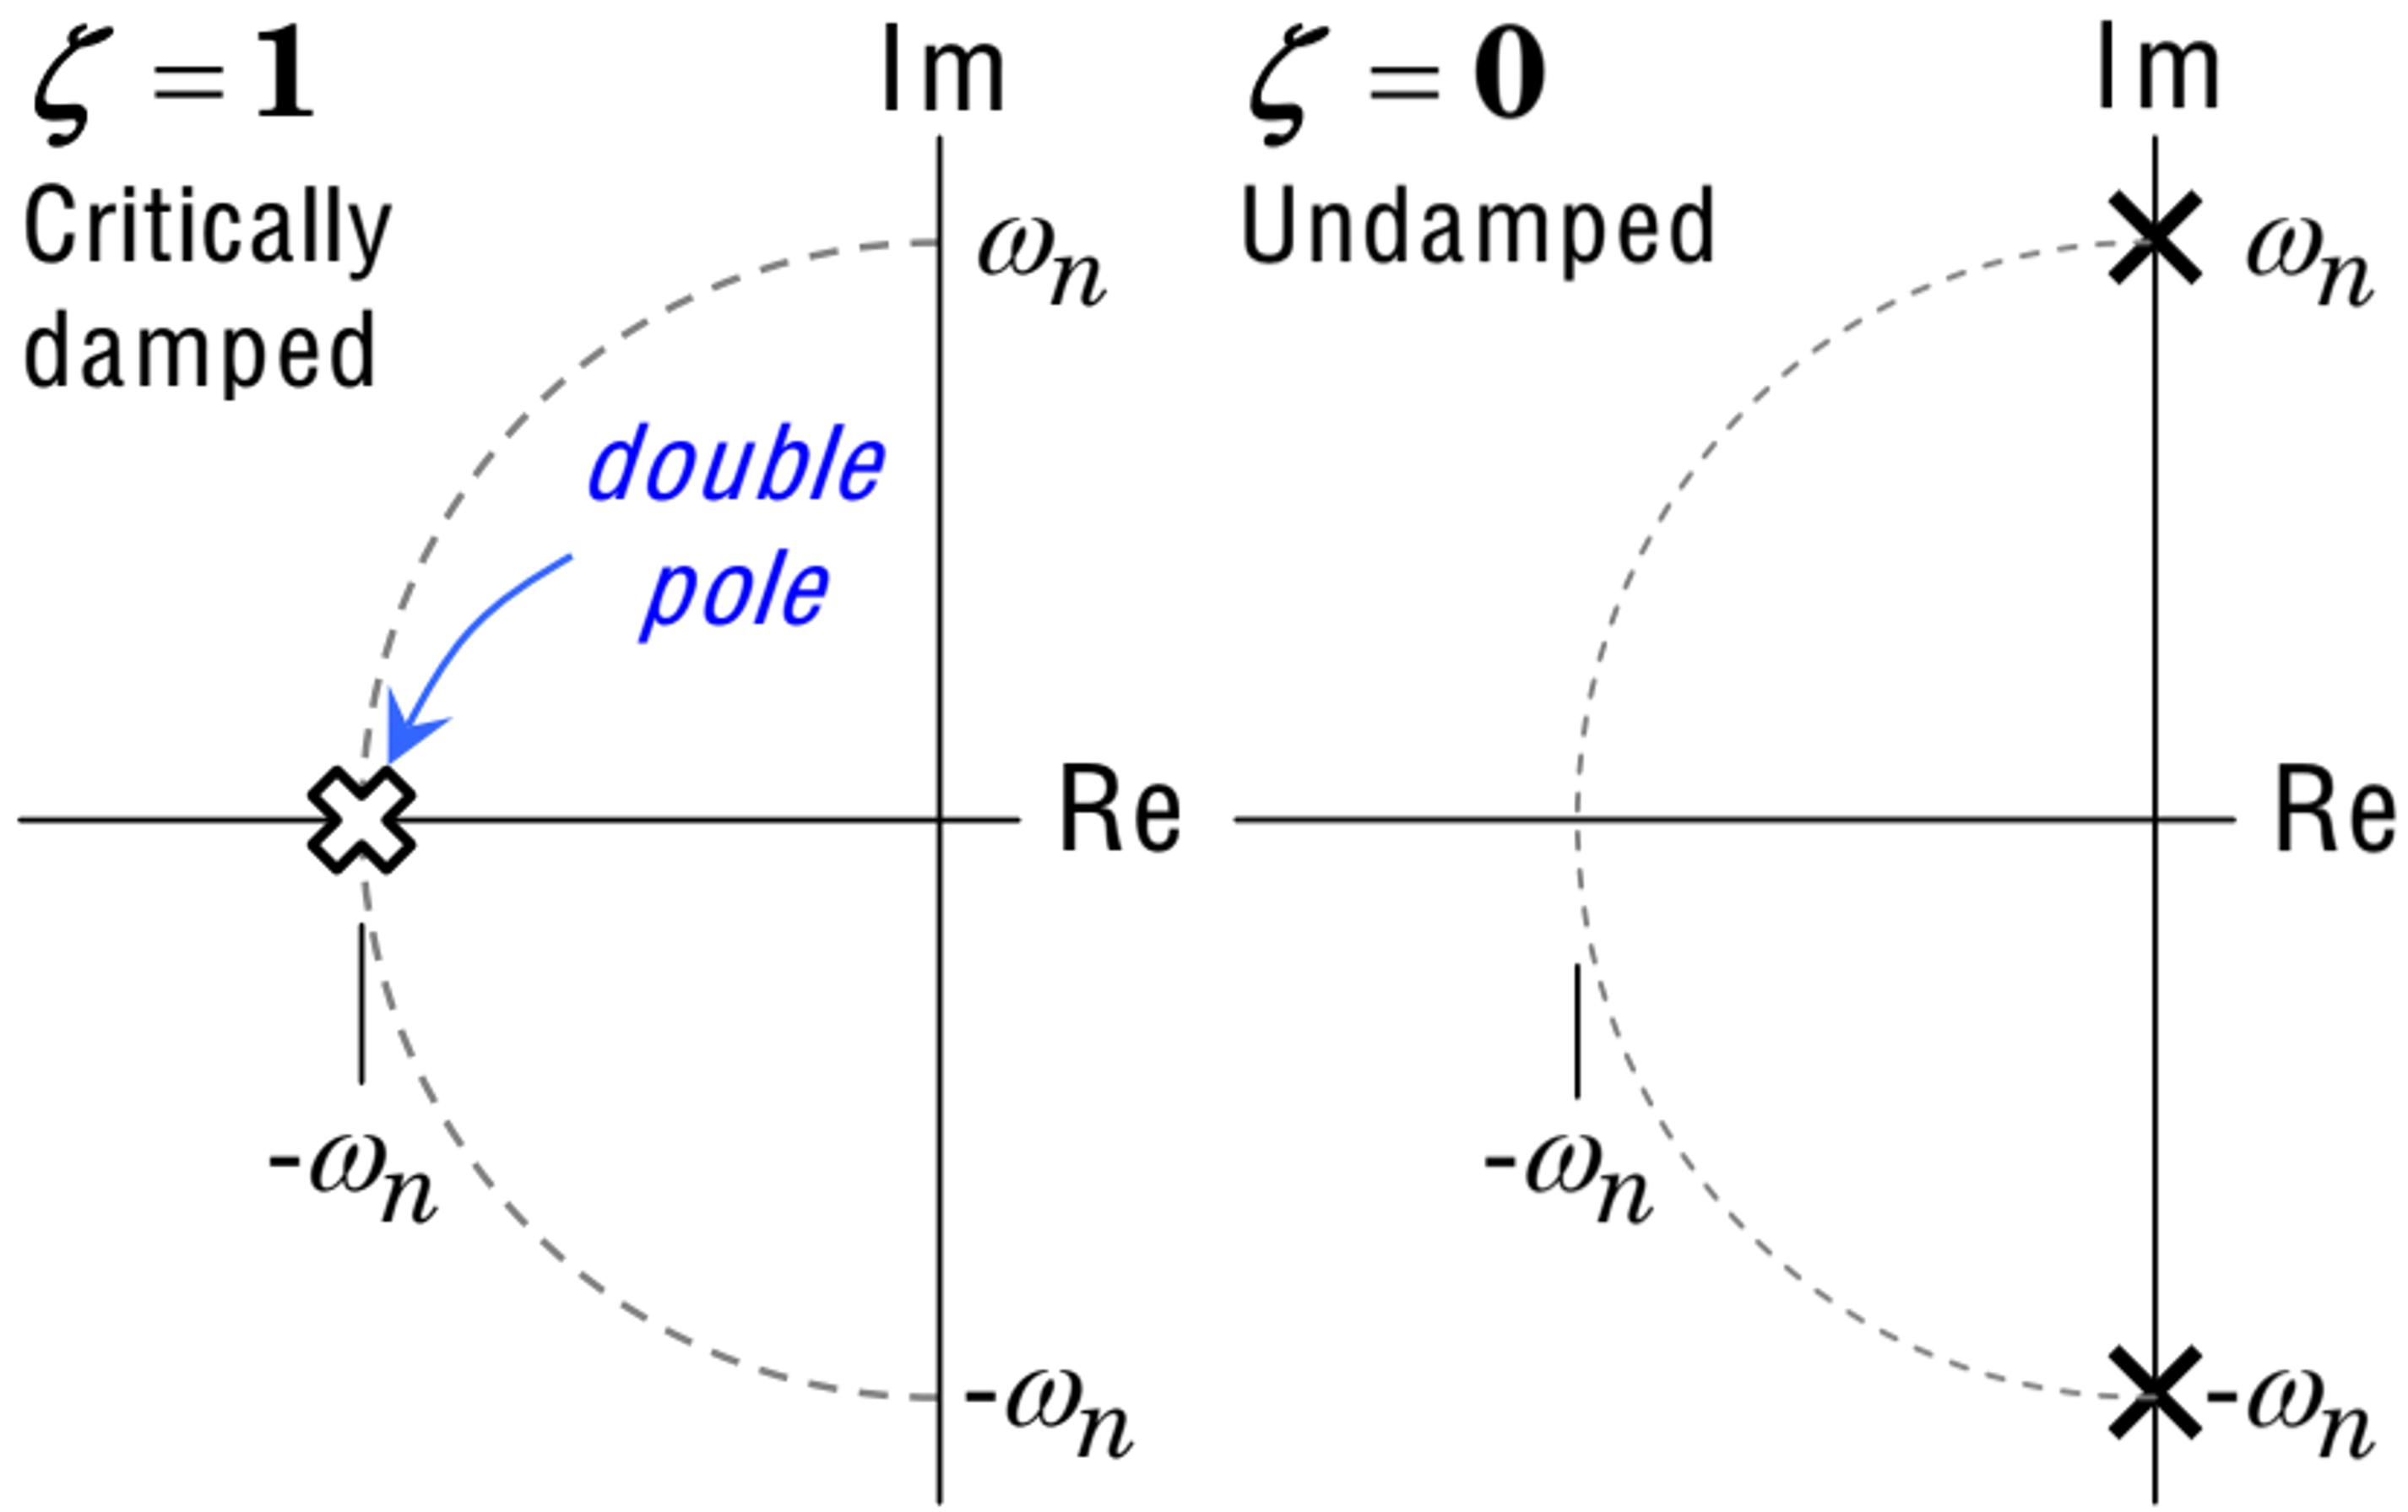
\includegraphics[width=\linewidth]{criticallyDamped_undamped.png}                
        % \end{Figure}
        % \begin{Figure}
        %     \centering
        %     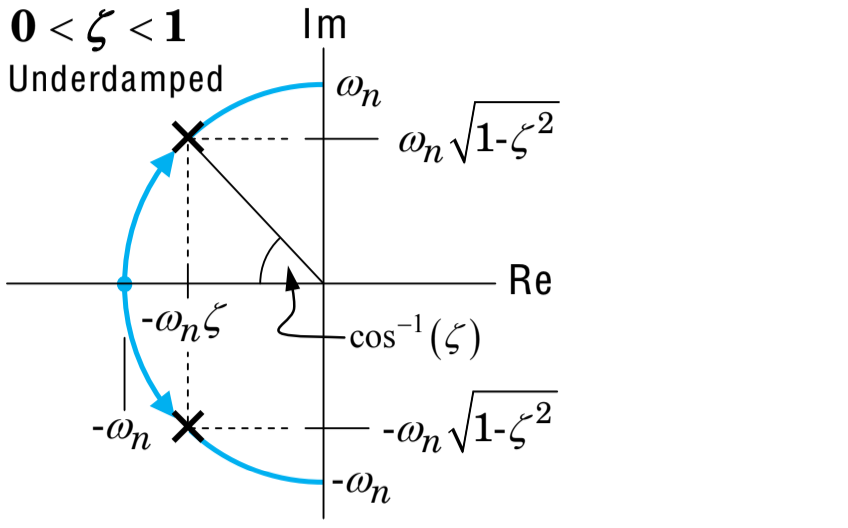
\includegraphics[width=\linewidth]{underdamped.png}                
        % \end{Figure}
    \end{itemize}
    
    \begin{itemize}
        \item Overdamped system: distinct real poles, $\zeta > 1$
        \item Critically damped system: repeated real poles, $\zeta = 1$
        \item Underdamped system: conjugate complex poles,\\$0 < \zeta < 1$
        \item Undamped system: conjugate imaginary poles, $\zeta = 0$
    \end{itemize}

    \textbf{\uline{Chapter 8}}

    % Bode plot: approximate visualization of frequency response, $\tilde{H}(j \omega)$ of a system
    % \begin{itemize}
    %     \item Magnitude plot: plot of $\left|\tilde{H}(j \omega)\right|_{dB} = 20 \log_{10}\left(\left|\tilde{H}(j \omega)\right|\right) dB$
    %     \item Phase plot: plot of $\angle \tilde{H}(j \omega)$ in degrees
    %     \item $x$-axis is logarithmically scaled (semilog-$x$: scale is log, but labels are still linear)
    %     \item Only positive frequency side visualized (which suffices for real systems as $|\tilde{H}(j \omega)|$ and $\angle \tilde{H}(j \omega)$ are even and odd functions of $\omega$ respectively)
    %     \item 0 is not in the axis cuz it goes from 1 to 0.1 to 0.01 to 0.001...
    % \end{itemize}

    \textbf{8.1 Construction of Bode Plots}

    % Need to express (7.23b) in a suitable form for each of the following cases:
    % \begin{itemize}
    %     \item Systems without integrator and differentiator
    %     \item Systems with differentiators
    %     \item Systems with integrators
    % \end{itemize}

    Basic systems:
    \begin{enumerate}
        \item $\tilde{H}(s) = K_{dc}$: DC gain (constant)
        \item $\tilde{H}(s) = K_d s$: differentiator with gain $K_d$
        \item $\tilde{H}(s) = K_i/s$: integrator with gain $K_i$
        \item $\tilde{H}(s) = s/z_m + 1$: zero factor with unity DC gain ($\tilde{H}(0) = 1$)
        \item $\tilde{H}(s) = \frac{1}{s/p_n + 1}$: pole factor with unity DC gain
        \item $\tilde{H}(s) = \frac{\omega_n^2}{s^2+2\zeta\omega_ns + \omega_n^2}$: 2nd-order factor with unity DC gain
    \end{enumerate}

    \leavevmode\\
    % \textbf{1. DC gain ($\tilde{H}(s) = K_{dc}$)}
    % \begin{Figure}
    %     \centering
    %     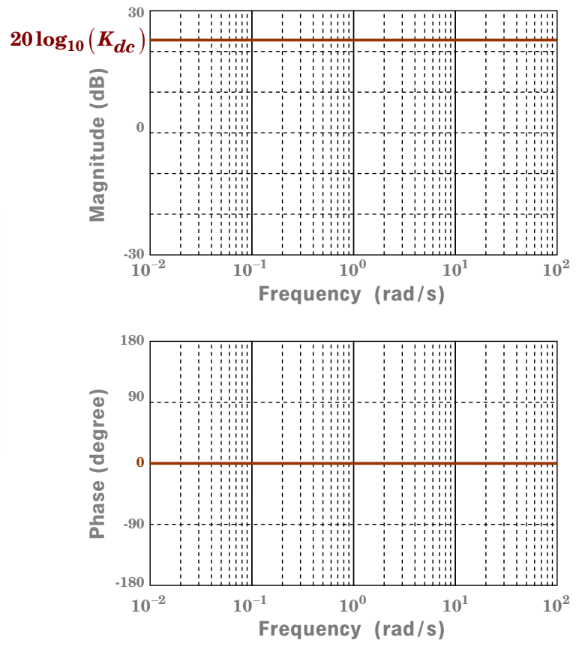
\includegraphics[width=\linewidth]{bode_dcGain.png}        
    % \end{Figure}

    % \textbf{2. Differentiator ($\tilde{H}(s) = K_d s$)}
    % \begin{Figure}
    %     \centering
    %     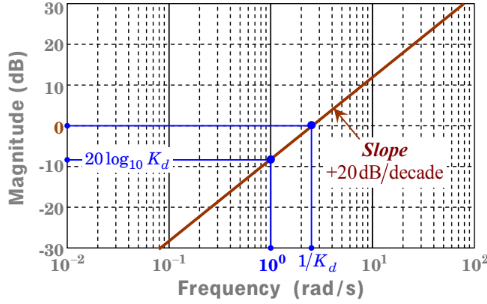
\includegraphics[width=\linewidth]{bode_differentiator1.png}        
    % \end{Figure}
    % \begin{Figure}
    %     \centering
    %     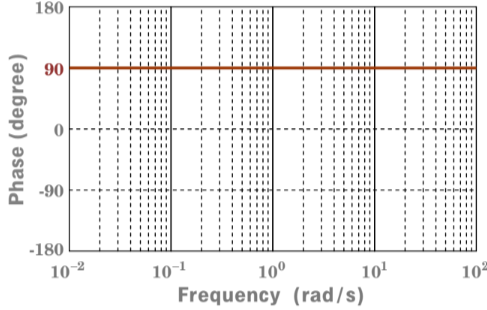
\includegraphics[width=\linewidth]{bode_differentiator2.png}        
    % \end{Figure}

    % \textbf{3. Integrator ($\tilde{H}(s) = K_i/s$)}
    % \begin{Figure}
    %     \centering
    %     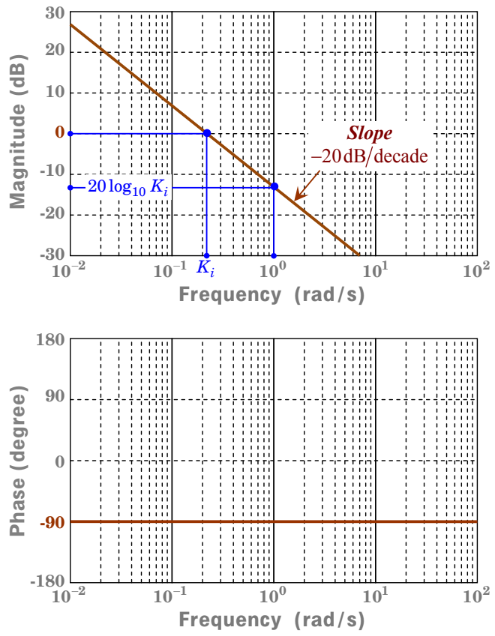
\includegraphics[width=\linewidth]{bode_integrator.png}        
    % \end{Figure}

    % \textbf{4. Zero factor ($\tilde{H}(s) = s/z_m + 1$)}
    % \begin{Figure}
    %     \centering
    %     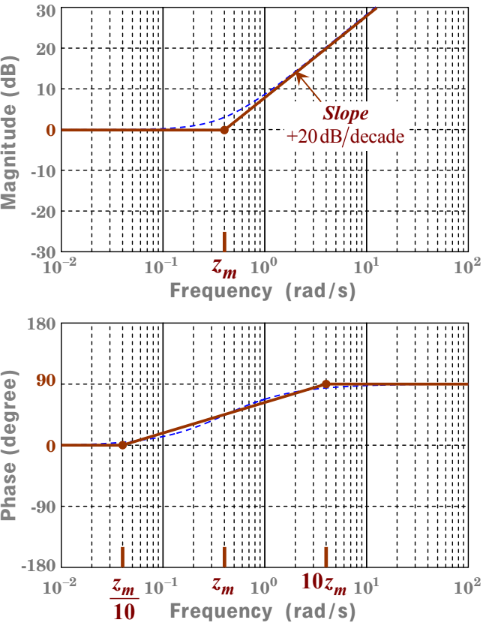
\includegraphics[width=\linewidth]{bode_zeroFactor.png}        
    % \end{Figure}

    % \textbf{5. Pole factor ($\tilde{H}(s) = \frac{1}{s/p_n + 1}$)}
    % \begin{Figure}
    %     \centering
    %     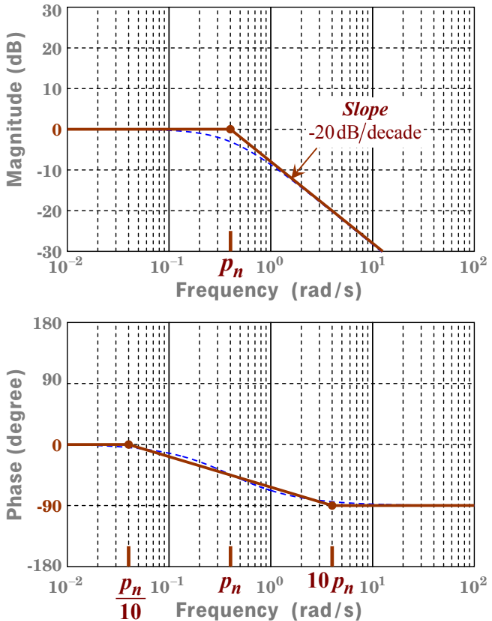
\includegraphics[width=\linewidth]{bode_poleFactor.png}        
    % \end{Figure}

    % \textbf{6. 2nd-order factor ($\tilde{H}(s) = \frac{\omega_n^2}{s^2+2\zeta\omega_ns + \omega_n^2}$)}
    % \begin{Figure}
    %     \centering
    %     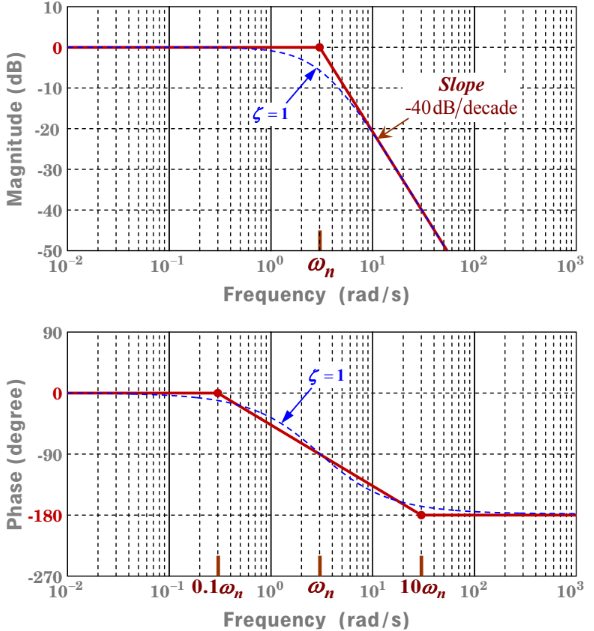
\includegraphics[width=\linewidth]{bode_2ndOrder.png}        
    % \end{Figure}

    \textbf{8.2 Asymptotic Behavior of Bode Plots}
    \begin{Figure}
        \centering
        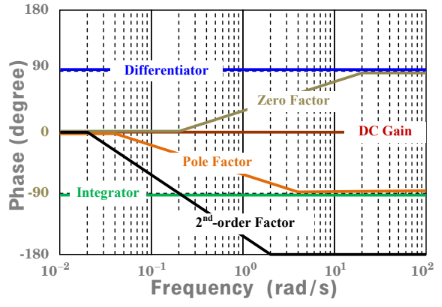
\includegraphics[width=\linewidth]{bode1.png}        
    \end{Figure}
    \begin{Figure}
        \centering
        \includegraphics[width=\linewidth]{bode2.png}        
    \end{Figure}

    \textbf{Asymptotic phase of phase plot}

    High frequency:
    \begin{align*}
        \text{Pole-zero excess} \times (-90 \degree) \tag{8.4a}
    \end{align*}

    Low frequency:
    \begin{align*}
        \left[\text{No. of }\int dt - \text{No. of } \frac{d}{dt}\right] \times (-90 \degree) \tag{8.4b}
    \end{align*}

    \textbf{Asymptotic slope of magnitude plot}

    High frequency:
    \begin{align*}
        [\text{Pole-zero excess}] \times (-20 \text{ dB/decade}) \tag{8.5a}
    \end{align*}

    Low frequency:
    \begin{align*}
        \left[\text{No. of} \int dt - \text{No. of } \frac{d}{dt}\right] \times (-20 \text{ dB/decade}) \tag{8.5a}
    \end{align*}

    \textbf{\uline{Chapter 9}}

    \textbf{\uline{9.1 Idealized LTI filters}}

    \textbf{Ideal Low-Pass Filter (LPF)}
    \begin{itemize}
        \item Frequency response: $H(f) = A\rect{\frac{f}{2B}}$
        \item Impulse response: $h(t) = 2AB\sinc{2Bt}$
    \end{itemize}

    % \begin{Figure}
    %     \centering
    %     \includegraphics[width=\linewidth]{idealLPF.png}
    % \end{Figure}

    \textbf{Ideal Band-Pass Filter (BPF)}
    \begin{itemize}
        \item Frequency response:\\
        $H(f) = A \left[\rect{\frac{f + f_0}{B}} + \rect{\frac{f - f_0}{B}}\right]$
        \item Impulse response:\\
        $h(t)=2AB\sinc{Bt}\cos{(2\pi f_0t)}$
    \end{itemize}

    % \begin{Figure}
    %     \centering
    %     \includegraphics[width=\linewidth]{idealBPF.png}
    % \end{Figure}

    \textbf{\uline{9.2 Continuous-time Sampling and\\Reconstruction of Signals}}

    % \textbf{Sampling}

    % \begin{Figure}
    %     \centering
    %     \includegraphics[width=\linewidth]{continuousTimeSampling.png}        
    % \end{Figure}

    % \textbf{Reconstruction}

    % \begin{Figure}
    %     \centering
    %     \includegraphics[width=\linewidth]{reconstruction.png}        
    % \end{Figure}

    \textbf{Nyquist Sampling Theorem:}
    % \begin{itemize}
    %     \item A band-limited signal, which has no frequency components higher than $f_m$ Hz ($f_m$ = bandwidth = highest freq component), may be completely described by specifying the values of the signal at insants of time separated by no more than $\frac{1}{2f_m}$ seconds.
    %     \item A band-limited signal, which has no frequency components higher than $f_m$ Hz, may be completely recovered from a knowledge of its samples taken at a rate of no less than $2 f_m$ samples/second.
    % \end{itemize}

    Nyquist sampling frequency / Nyquist rate $f_s = 2 f_m$

    \textbf{\uline{9.3 Sampling Band-limited Bandpass\\Signal below Nyquist Rate}}

    \begin{enumerate}[label=(\alph*)]
        \item Overlapping spectral images ($f_c > 0.5B$)
        \[
            f_s = 2f_c / k; \quad k = 1,2,\ldots, \lfloor 2f_c/B \rfloor \tag{9.2a}
        \]
        \item Un-aliased spectral images ($f_c > 1.5B$)

        \[
            \begin{split}
                \frac{2f_c + B}{k + 1} \leq f_s \leq \frac{2f_c - B}{k};\\
                k = 1,2,\ldots,\left\lfloor \frac{2f_c - B}{2B} \right\rfloor
            \end{split} \tag{9.2b}
        \]
    \end{enumerate}
\end{multicols*}
\end{document}
